\documentclass{book}
\usepackage{fontspec}
\setmainfont{STIX Two Text}

%PACKAGES
\iffalse
Here are the packages that I use
\fi

\usepackage{blindtext, hyperref, verbatim, minted, graphicx, amssymb, textcomp, enumerate, tcolorbox, newunicodechar, textgreek, wasysym, tipa, eso-pic, lipsum, bbold, dsfont}
\usepackage[margin=1.3in]{geometry}
\usepackage{longtable}
\usepackage{newunicodechar}
\usepackage{amsthm}
\usepackage{tikz}
\usepackage{tikz-cd}


\usepackage{lipsum} % for generating dummy text
\usepackage{draftwatermark} % for adding watermark
\usepackage{xcolor} % for colors

% Define the draft watermark
\SetWatermarkText{\textcolor{red}{ND}}
\SetWatermarkScale{2} % Adjust the size of the watermark





%ENVIRONMENTS

%Here I define some common environments. I use definitions, theorems, examples, and lemmas.


\theoremstyle{definition}
\newtheorem{definition}{Definition}
\newtheorem{theorem}{Theorem}
\newtheorem{example}{Example}
\newtheorem{lemma}{Lemma}


\newunicodechar{ₙ}{${}_{n}$}

\newunicodechar{𝓓}{$\mathcal{D}$}
\newunicodechar{∂}{$\partial$}

%\newunicodechar{π⃗}{$\stackrel{\arr}{\pi}$}

\newunicodechar{×}{$\times$}
\newunicodechar{→}{$\rightarrow$}
\newunicodechar{⟨}{$\langle$}
\newunicodechar{⟩}{$\rangle$}
\newunicodechar{↦}{$\mapsto$}
\newunicodechar{∧}{$\wedge$}
\newunicodechar{∨}{$\vee$}
\newunicodechar{∃}{$\exists$}
\newunicodechar{∀}{$\forall$}
\newunicodechar{¬}{$\neg$}
\newunicodechar{ᵃ}{${}^{\texttt{a}}$}
\newunicodechar{ᵇ}{${}^{\texttt{b}}$}
\newunicodechar{ᶜ}{${}^{\texttt{c}}$}
\newunicodechar{ᵈ}{${}^{\texttt{d}}$}
\newunicodechar{ᵉ}{${}^{\texttt{e}}$}
\newunicodechar{ᶠ}{${}^{\texttt{f}}$}
\newunicodechar{ᵍ}{${}^{\texttt{g}}$}
\newunicodechar{ʰ}{${}^{\texttt{h}}$}
\newunicodechar{ⁱ}{${}^{\texttt{i}}$}
\newunicodechar{ʲ}{${}^{\texttt{j}}$}
\newunicodechar{ᵏ}{${}^{\texttt{k}}$}
\newunicodechar{ˡ}{${}^{\texttt{l}}$}
\newunicodechar{ᵐ}{${}^{\texttt{m}}$}
\newunicodechar{ⁿ}{${}^{\texttt{n}}$}
\newunicodechar{ᵒ}{${}^{\texttt{o}}$}
\newunicodechar{ᵖ}{${}^{\texttt{ω}}$}
\newunicodechar{ʳ}{${}^{\texttt{r}}$}
\newunicodechar{ˢ}{${}^{\texttt{s}}$}
\newunicodechar{ᵗ}{${}^{\texttt{t}}$}
\newunicodechar{ᵘ}{${}^{\texttt{u}}$}
\newunicodechar{ᵛ}{${}^{\texttt{v}}$}
\newunicodechar{ʷ}{${}^{\texttt{w}}$}
\newunicodechar{ˣ}{${}^{\texttt{x}}$}
\newunicodechar{ʸ}{${}^{\texttt{y}}$}
\newunicodechar{ᶻ}{${}^{\texttt{z}}$}
\newunicodechar{⁰}{${}^{\texttt{0}}$}
\newunicodechar{¹}{${}^{\texttt{1}}$}
\newunicodechar{²}{${}^{\texttt{2}}$}
\newunicodechar{³}{${}^{\texttt{3}}$}
\newunicodechar{⁴}{${}^{\texttt{4}}$}
\newunicodechar{⁵}{${}^{\texttt{5}}$}
\newunicodechar{⁶}{${}^{\texttt{6}}$}
\newunicodechar{⁷}{${}^{\texttt{7}}$}
\newunicodechar{⁸}{${}^{\texttt{8}}$}
\newunicodechar{⁹}{${}^{\texttt{9}}$}
\newunicodechar{⁻}{${}^{\texttt{-}}$}
\newunicodechar{ᵒ}{${}^{\texttt{o}}$}
\newunicodechar{ᵖ}{${}^{\texttt{ω}}$}
\newunicodechar{⁻}{${}^{\texttt{-}}$}
\newunicodechar{¹}{${}^{\texttt{1}}$}
\newunicodechar{₀}{${}_{\texttt{0}}$}
\newunicodechar{₁}{${}_{\texttt{1}}$}
\newunicodechar{₂}{${}_{\texttt{2}}$}
\newunicodechar{₃}{${}_{\texttt{3}}$}
\newunicodechar{₄}{${}_{\texttt{4}}$}
\newunicodechar{₅}{${}_{\texttt{5}}$}
\newunicodechar{₆}{${}_{\texttt{6}}$}
\newunicodechar{₇}{${}_{\texttt{7}}$}
\newunicodechar{₈}{${}_{\texttt{8}}$}
\newunicodechar{₉}{${}_{\texttt{9}}$}
\newunicodechar{𝔸}{$\mathbb{A}$}
\newunicodechar{𝔹}{$\mathbb{B}$}
\newunicodechar{ℂ}{$\mathbb{C}$}
\newunicodechar{𝔻}{$\mathbb{D}$}
\newunicodechar{𝔼}{$\mathbb{E}$}
\newunicodechar{𝔽}{$\mathbb{F}$}
\newunicodechar{𝔾}{$\mathbb{G}$}
\newunicodechar{ℍ}{$\mathbb{H}$}
\newunicodechar{𝕀}{$\mathbb{I}$}
\newunicodechar{𝕁}{$\mathbb{J}$}
\newunicodechar{𝕂}{$\mathbb{K}$}
\newunicodechar{𝕃}{$\mathbb{L}$}
\newunicodechar{𝕄}{$\mathbb{M}$}
\newunicodechar{ℕ}{$\mathbb{N}$} 
\newunicodechar{𝕆}{$\mathbb{O}$}
\newunicodechar{ℙ}{$\mathbb{P}$}
\newunicodechar{ℚ}{$\mathbb{Q}$}
\newunicodechar{ℝ}{$\mathbb{R}$}
\newunicodechar{𝕊}{$\mathbb{S}$}
\newunicodechar{𝕋}{$\mathbb{T}$} 
\newunicodechar{𝕌}{$\mathbb{U}$}
\newunicodechar{𝕍}{$\mathbb{V}$}
\newunicodechar{𝕎}{$\mathbb{W}$}
\newunicodechar{𝕏}{$\mathbb{X}$}
\newunicodechar{𝕐}{$\mathbb{Y}$}
\newunicodechar{ℤ}{$\mathbb{Z}$}
\newunicodechar{𝕒}{$\mathbb{a}$}
\newunicodechar{𝕓}{$\mathbb{b}$}
\newunicodechar{𝕔}{$\mathbb{c}$}
\newunicodechar{𝕕}{$\mathbb{d}$}
\newunicodechar{𝕖}{$\mathbb{e}$}
\newunicodechar{𝕗}{$\mathbb{f}$}
\newunicodechar{𝕘}{$\mathbb{g}$}
\newunicodechar{𝕙}{$\mathbb{h}$}
\newunicodechar{𝕚}{$\mathbb{i}$}
\newunicodechar{𝕛}{$\mathbb{j}$}
\newunicodechar{𝕜}{$\mathbb{k}$}%𝔸𝔹ℂ𝔻𝔼𝔽𝔾ℍ𝕀𝕁𝕂𝕃𝕄ℕ𝕆ℙℚℝ𝕊𝕋𝕌𝕍𝕎𝕏𝕐ℤ𝕒𝕓𝕔𝕕𝕖𝕗𝕘𝕙𝕚𝕛𝕜𝕝𝕞𝕟𝕠𝕡𝕢𝕣𝕤𝕥𝕦𝕧𝕨𝕩𝕪𝕫
\newunicodechar{𝕝}{$\mathbb{l}$} 
\newunicodechar{𝕞}{$\mathbb{m}$}
\newunicodechar{𝕟}{$\mathbb{n}$}
\newunicodechar{𝕠}{$\mathbb{o}$}
\newunicodechar{𝕡}{$\mathbb{p}$}
\newunicodechar{𝕢}{$\mathbb{q}$}
\newunicodechar{𝕣}{$\mathbb{r}$}
\newunicodechar{𝕤}{$\mathbb{s}$}
\newunicodechar{𝕥}{$\mathbb{t}$}
\newunicodechar{𝕦}{$\mathbb{u}$}
\newunicodechar{𝕧}{$\mathbb{v}$}
\newunicodechar{𝕨}{$\mathbb{w}$}
\newunicodechar{𝕩}{$\mathbb{x}$}
\newunicodechar{𝕪}{$\mathbb{y}$}
\newunicodechar{𝕫}{$\mathbb{z}$}
\newunicodechar{𝚫}{$\Delta$}
\newunicodechar{ʃ}{$\int$}
\newunicodechar{∪}{$\cup$}
\newunicodechar{∩}{$\cap$}
\newunicodechar{±}{$\pm$}
\newunicodechar{𝔄}{$\mathfrak{A}$}




\newunicodechar{𝔅}{$\mathfrak{B}$}
\newunicodechar{ℭ}{$\mathfrak{C}$}
\newunicodechar{𝔇}{$\mathfrak{D}$}
\newunicodechar{𝔈}{$\mathfrak{E}$}
\newunicodechar{𝔉}{$\mathfrak{F}$}
\newunicodechar{𝔊}{$\mathfrak{G}$}
\newunicodechar{ℌ}{$\mathfrak{H}$}
\newunicodechar{ℑ}{$\mathfrak{I}$}
\newunicodechar{𝔍}{$\mathfrak{J}$}
\newunicodechar{𝔎}{$\mathfrak{K}$}
\newunicodechar{𝔏}{$\mathfrak{L}$}
\newunicodechar{𝔐}{$\mathfrak{M}$}
\newunicodechar{𝔑}{$\mathfrak{N}$}
\newunicodechar{𝔒}{$\mathfrak{O}$}
\newunicodechar{𝔓}{$\mathfrak{P}$}
\newunicodechar{𝔔}{$\mathfrak{Q}$}
\newunicodechar{ℜ}{$\mathfrak{R}$}
\newunicodechar{𝔖}{$\mathfrak{S}$}
\newunicodechar{𝔗}{$\mathfrak{T}$}
\newunicodechar{𝔘}{$\mathfrak{U}$}
\newunicodechar{𝔙}{$\mathfrak{V}$}
\newunicodechar{𝔚}{$\mathfrak{W}$}
\newunicodechar{𝔛}{$\mathfrak{X}$}
\newunicodechar{𝔜}{$\mathfrak{Y}$}
\newunicodechar{ℨ}{$\mathfrak{Z}$}

\newunicodechar{𝔞}{$\mathfrak{a}$}
\newunicodechar{𝔟}{$\mathfrak b$}
\newunicodechar{𝔠}{$\mathfrak{c}$}
\newunicodechar{𝔡}{$\mathfrak{d}$}
\newunicodechar{𝔢}{$\mathfrak{e}$}
\newunicodechar{𝔣}{$\mathfrak{f}$}
\newunicodechar{𝔤}{$\mathfrak{g}$}
\newunicodechar{𝔥}{$\mathfrak{h}$}
\newunicodechar{𝔦}{$\mathfrak{i}$}
\newunicodechar{𝔧}{$\mathfrak{j}$}
\newunicodechar{𝔨}{$\mathfrak{k}$}
\newunicodechar{𝔩}{$\mathfrak{l}$}
\newunicodechar{𝔪}{$\mathfrak{m}$}
\newunicodechar{𝔫}{$\mathfrak{n}$}
\newunicodechar{𝔬}{$\mathfrak{o}$}
\newunicodechar{𝔭}{$\mathfrak{ω}$}
\newunicodechar{𝔮}{$\mathfrak{q}$}
\newunicodechar{𝔯}{$\mathfrak{r}$}
\newunicodechar{𝔰}{$\mathfrak{s}$}
\newunicodechar{𝔱}{$\mathfrak{t}$}
\newunicodechar{𝔲}{$\mathfrak{u}$}
\newunicodechar{𝔳}{$\mathfrak{v}$}
\newunicodechar{𝔴}{$\mathfrak{w}$}
\newunicodechar{𝔵}{$\mathfrak{x}$}
\newunicodechar{𝔶}{$\mathfrak{y}$}
\newunicodechar{𝔷}{$\mathfrak{z}$}

\newunicodechar{𝐀}{${\bf{A}}$}
\newunicodechar{𝐁}{${\bf{B}}$}
\newunicodechar{𝐂}{${\bf{C}}$}
\newunicodechar{𝐃}{${\bf{D}}$}
\newunicodechar{𝐄}{${\bf{E}}$}
\newunicodechar{𝐅}{${\bf{F}}$}
\newunicodechar{𝐆}{${\bf{G}}$}
\newunicodechar{𝐇}{${\bf{H}}$}
\newunicodechar{𝐈}{${\bf{I}}$}
\newunicodechar{𝐉}{${\bf{J}}$}
\newunicodechar{𝐊}{${\bf{K}}$}
\newunicodechar{𝐋}{${\bf{L}}$}
\newunicodechar{𝐌}{${\bf{M}}$}
\newunicodechar{𝐍}{${\bf{N}}$}
\newunicodechar{𝐎}{${\bf{O}}$}
\newunicodechar{𝐏}{${\bf{P}}$}
\newunicodechar{𝐐}{${\bf{Q}}$}
\newunicodechar{𝐑}{${\bf{R}}$}
\newunicodechar{𝐒}{${\bf{S}}$}
\newunicodechar{𝐓}{${\bf{T}}$}
\newunicodechar{𝐔}{${\bf{U}}$}
\newunicodechar{𝐕}{${\bf{V}}$}
\newunicodechar{𝐖}{${\bf{W}}$}
\newunicodechar{𝐗}{${\bf{X}}$}
\newunicodechar{𝐘}{${\bf{Y}}$}
\newunicodechar{𝐙}{${\bf{Z}}$}

\newunicodechar{𝐚}{${\bf{a}}$}
\newunicodechar{𝐛}{${\bf{b}}$}
\newunicodechar{𝐜}{${\bf{c}}$}
\newunicodechar{𝐝}{${\bf{d}}$}
\newunicodechar{𝐞}{${\bf{e}}$}
\newunicodechar{𝐟}{${\bf{f}}$}
\newunicodechar{𝐠}{${\bf{g}}$}
\newunicodechar{𝐡}{${\bf{h}}$}
\newunicodechar{𝐢}{${\bf{i}}$}
\newunicodechar{𝐣}{${\bf{j}}$}
\newunicodechar{𝐤}{${\bf{k}}$}
\newunicodechar{𝐥}{${\bf{l}}$}
\newunicodechar{𝐦}{${\bf{m}}$}
\newunicodechar{𝐧}{${\bf{n}}$}
\newunicodechar{𝐨}{${\bf{o}}$}
\newunicodechar{𝐩}{${\bf{ω}}$}
\newunicodechar{𝐪}{${\bf{q}}$}
\newunicodechar{𝐫}{${\bf{r}}$}
\newunicodechar{𝐬}{${\bf{s}}$}
\newunicodechar{𝐭}{${\bf{t}}$}
\newunicodechar{𝐮}{${\bf{u}}$}
\newunicodechar{𝐯}{${\bf{v}}$}
\newunicodechar{𝐰}{${\bf{w}}$}
\newunicodechar{𝐱}{${\bf{x}}$}
\newunicodechar{𝐲}{${\bf{y}}$}
\newunicodechar{𝐳}{${\bf{z}}$}

\newunicodechar{⊣}{\ensuremath{\dashv}}
\newunicodechar{ॱ}{${}^{\cdot}$}
\newunicodechar{𛲔}{${}_{\cdot}$}
\newunicodechar{⋯}{$\cdots$}
\newunicodechar{⇄}{$\rightleftarrows$}
\newunicodechar{⇆}{$\leftrightarrows$}

\newunicodechar{ꜝ}{$\raisebox{1ex}{\scalebox{0.5}{\texttt{!}}}$}
\newunicodechar{ꜞ}{$\raisebox{1ex}{\scalebox{0.5}{\texttt{¡}}}$}



%This is notation we will use for categories


\newunicodechar{𝟙}{$\mathbb{1}$}
\newunicodechar{∘}{$\circ$}

%This is notation we will use for twocategories


\newunicodechar{𝟏}{${\bold{1}}$}
\newunicodechar{⭢}{$\longrightarrow$}
\newunicodechar{•}{${\bullet}$}
\newunicodechar{∙}{${\bullet}$}

%This is notation we will use for ∞-ℂ𝕒𝕥

\newunicodechar{よ}{$
\includegraphics[width=0.27cm,height=0.27cm]{yon.png}$}
\newunicodechar{⊥}{$\bot$}
\newunicodechar{∼}{$\sim$}
\newunicodechar{≃}{$\simeq$}
\newunicodechar{≅}{$\cong$}
\newunicodechar{∞}{$\infty$}

\newunicodechar{α}{$\alpha$}
\newunicodechar{β}{$\beta$}
\newunicodechar{γ}{$\gamma$}
\newunicodechar{δ}{$\delta$}
\newunicodechar{ε}{$\epsilon$}
\newunicodechar{η}{$\eta$}
\newunicodechar{ζ}{$\zeta$}
\newunicodechar{θ}{$\theta$}
\newunicodechar{ι}{$\iota$}
\newunicodechar{μ}{$\mu$}
\newunicodechar{κ}{$\kappa$}
\newunicodechar{λ}{$\lambda$}
\newunicodechar{ρ}{$\rho$}
\newunicodechar{π}{$\pi$}
\newunicodechar{σ}{$\sigma$}
\newunicodechar{τ}{$\tau$}
\newunicodechar{υ}{$\upsilon$}
\newunicodechar{φ}{$\phi$}
\newunicodechar{ψ}{$\psi$}
\newunicodechar{ξ}{$\xi$}
\newunicodechar{χ}{$\chi$}
\newunicodechar{ω}{$\omega$}

\newunicodechar{⊗}{$\otimes$}

\makeatletter
\newcommand*{\shifttext}[2]{\settowidth{\@tempdima}{#2}\makebox[\@tempdima]{\hspace*{#1}#2}}
\makeatother
\definecolor{Red}{cmyk}{0.1, 0.70, 0.65, 0.00, 1.00}
\definecolor{Blue}{cmyk}{0.9, 0.2, 0.2, 0.00, 1.00}
\definecolor{Yellow}{cmyk}{0.0, 0.00, 0.7, 0.00, 0.5}
\definecolor{Green}{cmyk}{0.6, 0.0, 0.6, 0.00, 1.00}
\definecolor{Purple}{cmyk}{0.8, 0.3, 0.3, 0.00, 1.00}
\definecolor{Orange}{cmyk}{0.0, 0.3, 0.7, 0.00, 1.00}
\definecolor{Grey}{cmyk}{0.13, 0.13, 0.13, 0.00, 1.00}
\newcounter{definitioncounter}
\setcounter{definitioncounter}{1}
\newcounter{theoremcounter}
\setcounter{theoremcounter}{1}
\newcounter{printcounter}
\setcounter{printcounter}{1}
\newcounter{examplecounter}
\setcounter{examplecounter}{1}
\newcounter{ccounter}
\setcounter{ccounter}{1}
\newcounter{pcounter}
\setcounter{pcounter}{1}
\newcounter{lcounter}
\setcounter{lcounter}{1}
\newcounter{sectioncount}
\newcounter{subsectioncount}
\setcounter{sectioncount}{1}
\renewcommand{\section}[1]{\newpage\ \\ \ \\ \begin{center} \scalebox{1.5}{\texttt{\thesectioncount . #1}} \stepcounter{sectioncount} \setcounter{subsectioncount}{1} \end{center} \begin{center} \ \\ \ \\ \thispagestyle{empty} \end{center}}
\renewcommand{\subsection}[1]{\texttt{\thesubsectioncount . #1} \stepcounter{subsectioncount}}
\renewcommand{\backslash}{\reflectbox{\texttt{/}}}

\newcounter{chaptercount}
\renewcommand{\chapter}[1]{
\newpage
{
\Huge 
\begin{center}
\ \\
\ \\
\thispagestyle{empty}
\texttt{#1}
\end{center}}
\ \\
\ \\
}

\newcounter{partcount}
\stepcounter{partcount}
\renewcommand{\part}[1]{
\newpage
{
\Huge 
\begin{center}
\ \\
\ \\
\ \\
\ \\
\ \\
\ \\
\thispagestyle{empty}
\texttt{PART {\thepartcount}: #1}
\stepcounter{partcount}
\end{center}}
\ \\
\ \\
}


\begin{document}

\thispagestyle{empty} 

\AddToShipoutPicture*
    {\put(540,720){

    \href{http://www.linearlibrary.net}{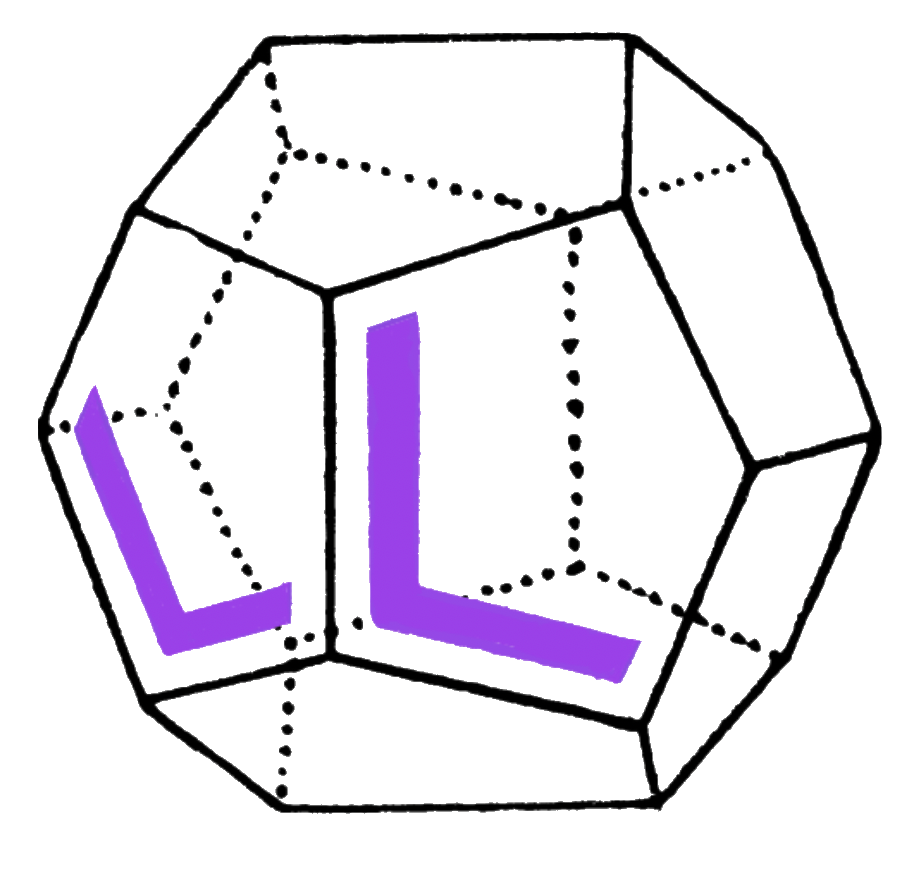
\includegraphics[width=2cm,height=2cm]{ll.png}}

    }}

\AddToShipoutPicture*
  {\put(470,767){
    \href{https://github.com/linlib/InfinitySpaces/StringDiagramGenerator.py}{\texttt{.py file}}
  }}

\AddToShipoutPicture*
  {\put(470,752){
    \href{https://github.com/linlib/InfinitySpaces/InfinitySpaces.tex}{\texttt{.tex file}}\\

  }}

\AddToShipoutPicture*
  {\put(470,737){

    \href{http://linearlibrary.net/InfinitySpaces/InfinitySpaces.pdf}{\texttt{.pdf file}}\\

  }}

  \AddToShipoutPicture*
  {\put(470,722){
    \href{https://github.com/linlib/InfinitySpaces/InfinitySpaces.lean}{\texttt{.lean file}}

  }}

\ \\

%LEAN: 
\begin{center}
\begin{tcolorbox}[width=2.3in,colback={white},coltitle=white]
\begin{center}
\ \\
\scalebox{3}{\texttt{∞-Spaces}}\\
\end{center}
\end{tcolorbox}
\end{center}
\ \\
\ \\
\ \\





\thispagestyle{empty}


\newpage


\begin{center}

\pagecolor{white}
\color{black}

\end{center}

\thispagestyle{empty}




\newpage
\pagecolor{white}
\color{black}
\ \\
\ \\
\thispagestyle{empty}
\begin{center}
Copyright\ \textcopyright \ October 19th 2023 Elliot Dean Young and Jiazhen Xia.\ All rights reserved.\\
\end{center}
\large %%%%%%%% HERE IS THE large LARGE size textsize set text size
\newpage 
\ \\
\ \\
\ \\
\ \\
\ \\
\ \\
\ \\
\ \\
\ \\
\ \\
\ \\
\thispagestyle{empty}
 
\newpage

\ \\
\ \\
\ \\
\ \\
\ \\
\ \\
\ \\
\ \\
\ \\
\ \\
\ \\

We wish to acknowledge the collaborative efforts of E. Dean Young and Jiazhen Xia. Dean Young initially formulated the introduction with twelve goals, posting them on the Lean Zulip in August of 2023. Together the authors are pursuing these plans as a long term project.\\

\newpage

\section{Introduction}

In this document I would like to develop a construction of the classifying space functor which can be applied indefinitely, B¹. I will write Bⁿ for the n-fold composition of B¹. In ```TheWhiteheadTheoremandTwoVariations''', we developed two models of ∞-Grpd\_(A) and ∞-Grpd\_(B). These will produce two models on which B¹ can be defined:

\begin{enumerate}[(i)]
\item B¹ : OperadicGroup • OperadicGroup ∞-Grpd\_(A) ⭢ OperadicGroup • OperadicGroup ∞-Grpd\_(A)
\item B¹ : OperadicGroup • OperadicGroup ∞-Grpd\_(B) ⭢ OperadicGroup • OperadicGroup ∞-Grpd\_(B)
\end{enumerate} 

∞-Spaces ...

explore derivations and connections.

In this section, which makes use of the previous section concerning Haar integral, I intend to cover the ordinary versions of Poincare duality, Pontrjagin duality, and Fourier duality, as well as versions of these theorems using language enabled by the previous repositories. This won't culminate until far into the future, so for now I have jotted down some sketches.\\

\iffalse
https://redprl.org/
agda
rzk (new!)
\fi

\iffalse
https://mathoverflow.net/questions/464176/bⁿ-and-coherence
\fi

after this we develop chain complexes of these.\\

The table of contents below reflects the tentative long-term goals of the authors, with the main goal the pursuit of the Whitehead theorem for a point-set model involving Mathlib's predefined homotopy groups.\\

\begin{enumerate}
\item cup and cap product
\end{enumerate}

Ideas for future applications:

\begin{enumerate}
\item \url{https://arxiv.org/pdf/2206.13563.pdf}
\end{enumerate}

\begin{enumerate}
\item One of the basic things I wanted out of this was homotopy colimit preserving maps (Eⁱⁿᶠ-Alg A)ᵒᵖ ⭢ ∞-Grpd
\end{enumerate}



\section{Contents}

The contents below reflect most or all of the contents of each chapter, each of which is adds a fairly minimal .

{
\footnotesize
\begin{longtable}{|| l || l ||} 
\hline
\multicolumn{1}{||c||}{$\texttt{Section}$} & \multicolumn{1}{|c||}{$\texttt{Description}$} \\
\hline
\hline
Unfinished & \\
\hline
Contents & \\
\hline
Unicode & \\
\hline
Introduction & \\
\hline \hline
\multicolumn{2}{||c||}{\texttt{PART I: } ∞-SPACES} \\
\hline \hline
 \multicolumn{2}{||c||}{\texttt{Chapter 1: }Abelian Groups} \\
\hline \hline
abelian\_group & The type of abelian groups \\
\hline
AbelianGroup & The category of abelian groups \\
\hline \hline
 \multicolumn{2}{||c||}{\texttt{Chapter 2: }∞-Spaces} \\
\hline \hline
∞-space & ∞-spaces are... \\
 \hline
∞-Space & the category of ∞-spaces ... \\
\hline \hline
\multicolumn{2}{||c||}{\texttt{Chapter 3: }Tensor Product of Abelian Groups} \\
\hline \hline
- ⊗\_(AbelianGroups) - & Mathlib's tensor product of abelian groups \\
\hline
[-,-]\_(AbelianGroups) & Mathlib's hom of abelian groups\\
\hline \hline
\multicolumn{2}{||c||}{\texttt{Chapter 4: }Tensor Product of ∞-Spaces} \\
\hline \hline
- ⊗\_(∞-Space) - &  \\
\hline
[-,-]\_(∞-Space) &  \\
\hline \hline
\multicolumn{2}{||c||}{\texttt{Chapter 5: }Rings and Commutative Rings} \\
\hline \hline
ring & The type of rings \\
 \hline
Ring & The category of rings \\
 \hline \hline
  \multicolumn{2}{||c||}{\texttt{Chapter 6: }A${}^{\infty}$-Rings and E${}^{\infty}$-Rings} \\
\hline \hline
A${}^{\infty}$-ring & The type of A${}^{\infty}$-rings \\
\hline
A${}^{\infty}$-Ring & The category of A${}^{\infty}$-Rings \\
 \hline
E${}^{\infty}$-ring  & The type of E${}^{\infty}$-rings \\
 \hline
E${}^{\infty}$-Ring  & The category of E${}^{\infty}$-Rings \\
 \hline \hline
\multicolumn{2}{||c||}{\texttt{Chapter 7: }Modules and Modules over Commutative Rings} \\
\hline \hline
 &  \\
 \hline
 &  \\
 \hline \hline
\multicolumn{2}{||c||}{\texttt{Chapter 8: }A${}^{\infty}$-Modules and E${}^{\infty}$-Modules} \\
\hline \hline
A∞-Mod &  \\
\hline
A∞-Mod &  \\
 \hline \hline
 \multicolumn{2}{||c||}{\texttt{Chapter 9: }Set ⇄ Ab} \\
\hline \hline
Sॱ & The free abelian group functor \\
 \hline
S𛲔 & The forgetful functor from abelian groups to sets \\
 \hline
 &  \\
\hline \hline
 \multicolumn{2}{||c||}{\texttt{Chapter 10: }∞-Grpd ⇄ ∞-Space} \\
\hline \hline
 & The free ∞-space given an ∞-groupoid \\
\hline
 & The underlying ∞-groupoid of an ∞-space \\
\hline \hline
\multicolumn{2}{||c||}{\texttt{PART II: } DERIVATIONS AND CONNECTIONS} \\
\hline \hline
\multicolumn{2}{||c||}{\texttt{Chapter 11: }Lie Algebras} \\
\hline \hline
 &  \\
\hline \hline
\multicolumn{2}{||c||}{\texttt{Chapter 12: }Derivations} \\
\hline \hline
derivation & Definition of a derivation \\
\hline
\hline \hline
\multicolumn{2}{||c||}{\texttt{Chapter 13: }L${}^{\infty}$ Algebras} \\
\hline \hline
 &  \\
\hline \hline
\multicolumn{2}{||c||}{\texttt{Chapter 14: }∞-Derivations} \\
\hline \hline
∞-derivation & Definition of ??? \\
\hline \hline
\multicolumn{2}{||c||}{\texttt{Chapter 15: }Tensor Product of Lie Algebras} \\
\hline \hline
- ⊗\_(∞-Space) - &  \\
\hline
[-,-]\_(∞-Space) &  \\
\hline \hline
\multicolumn{2}{||c||}{\texttt{Chapter 16: }Tensor Product of L${}^{\infty}$-Algebras} \\
\hline \hline
ring & The type of rings \\ 
 \hline
Ring & The category of rings \\
 \hline \hline
\multicolumn{2}{||c||}{\texttt{Chapter 17: }Lie Algebra Representations} \\
\hline \hline
 & \\
\hline
 & \\
\hline \hline
\multicolumn{2}{||c||}{\texttt{Chapter 18: }Connections} \\
\hline \hline
 & \\
\hline
 & \\
\hline \hline
\multicolumn{2}{||c||}{\texttt{Chapter 19: }L${}^{\infty}$-Representations} \\
\hline \hline
 & \\
\hline
 & \\
\hline \hline
\multicolumn{2}{||c||}{\texttt{Chapter 20: }∞-Connections} \\
\hline \hline
 & \\
\hline
 & \\
\hline \hline
\multicolumn{2}{||c||}{\texttt{Chapter 21: }Tensor Product of Lie-Algebra Representations} \\
\hline \hline
- ⊗\_(∞-Space) - &  \\
\hline
[-,-]\_(∞-Space) &  \\
\hline \hline
\multicolumn{2}{||c||}{\texttt{Chapter 22: }Tensor Product of L${}^{\infty}$-Representations} \\
\hline \hline
ring & The type of rings \\
 \hline
Ring & The category of rings \\
 \hline \hline
\end{longtable}
}




\part{PART I: ABELIAN GROUPS AND ∞-SPACES}

{
\footnotesize
\begin{center}
\begin{tabular}{||l || l || l || l ||} 
 \hline
  \multicolumn{4}{||c||}{\texttt{Eight Structures}} \\
 \hline
 \multicolumn{2}{||c||}{\texttt{Strict}}  &  \multicolumn{2}{||c||}{\texttt{Lax}} \\
 \hline
 \texttt{Unitial} &  \texttt{Actional}  &  \texttt{Unitial} &  \texttt{Actional}\\
 \hline \hline
 \texttt{InternalMonoid}  & \texttt{InternalMonoidAction} & \texttt{A}${}^{\infty}$ & \texttt{OperadicMonoidAction} \\ 
 \hline
 \texttt{InternalCommutative Monoid} & \texttt{InternalCommutativeMonoidAction} & \texttt{OperadicMonoid} & \texttt{OperadicMonoidAction} \\
 \hline
\end{tabular}
\end{center}
}


\newpage
\chapter{Abelian Groups}

In this chapter I cover the type of abelian groups as well as the category of abelian groups.\\

\begin{enumerate}
\item Mathlib.Algebra.Group.Defs
\end{enumerate}



\newpage
\chapter{∞-Spaces}

∞-spaces have a negation:



For example, ... is operadic groups in operadic groups in O².\\


\begin{center}
OperadicGroup² ∞\_(∞-Grpd)
\end{center}

\iffalse
In the repository concerning classifying spaces, I . 

In the repository

OperadicCategory² ∞-Cat, OperadicGroupoid² ∞-Grpd, and OperadicGroup² ∞-Grpd
\fi

Could ∞-spaces be operadic groups in operadic groups?

\iffalse
B¹.obj (M × N) ⭢ (B¹.obj M) × (B¹.obj N)
\fi

\iffalse
B¹.obj (M × N) ⭢ (B¹.obj M) × (B¹.obj N)
gives

\fi

\iffalse
- Embedding Ringᵒᵖ              into ∞-presheaves in ∞-spaces
- Embedding DistributiveLattice into ∞-presheaves in ∞-spaces
- Embedding Scheme              into ∞-presheaves in ∞-spaces
https://leanprover.zulipchat.com/#narrow/stream/287929-mathlib4/topic/Definition.20of.20group.20scheme.3F
\fi


Abelian groups are internal groups in internal groups.



\newpage
\chapter{Tensor Product}

\begin{enumerate}
\item \iffalse https://leanprover-community.github.io/mathlib4_docs/Mathlib/LinearAlgebra/TensorProduct/Basic.html#TensorProduct \fi
\end{enumerate}


\newpage
\chapter{Smash Product of ∞-Spaces}

\iffalse
∧\_(∞-Spc)
\fi


\newpage
\chapter{Rings and Commutative Rings}




\newpage
\chapter{A${}^{\infty}$-Rings and E${}^{\infty}$-Rings}

make sure to include Alg

\iffalse
Besides that my ∞-spaces are different, I would like to make my Ainfinity and Einfinity objects as similar as possible.
\fi

make sure to include ∞-Alg...

\iffalse
- Embedding Ringᵒᵖ into ∞-presheaves in ∞-spaces
\fi

\iffalse
https://leanprover.zulipchat.com/#narrow/stream/116395-maths/topic/Ext.20and.20Tor
\fi

\iffalse
https://leanprover.zulipchat.com/#narrow/stream/116395-maths/topic/CDGAs
\fi

\iffalse
https://leanprover.zulipchat.com/#narrow/stream/116395-maths/topic/Tensor.20products.20of.20graded.20objects.20.2F.20chain.20complexes
\fi


\newpage
\chapter{Modules over Rings and Commutative Rings}




\newpage
\chapter{A${}^{\infty}$-Modules and E${}^{\infty}$-Modules}




\newpage
\chapter{Set₋₁ ⇄ AbelianGroup}

{
\footnotesize
\begin{center}
\begin{tabular}{||l ||} 
 \hline
Set ⇄ AbelianGroup \\
 \hline
\end{tabular}
\end{center}
}

Abelian groups are internal groups in internal groups in sets.\\



\newpage
\chapter{∞-Grpd₋₁ ⇄ OperadicGroup²}


{
\footnotesize
\begin{center}
\begin{tabular}{|| l ||} 
 \hline
∞-Grpd₋₁ ⇄ OperadicGroup² \\
 \hline
\end{tabular}
\end{center}
}

\begin{enumerate}
\item πₙ of an ∞-space arising from an ∞-groupoid
\item Hₙ of an 
\item Dold-Thom theorem
\item \iffalse https://leanprover.zulipchat.com/#narrow/stream/116395-maths/topic/homology \fi
\item B is iterable on this
\item Chn ... 
\item μ : Chn × Chn ⭢ Chn
\end{enumerate}





\part{PART II: DERIVATIONS AND CONNECTIONS}


\newpage
\chapter{Lie Algebras}




\newpage
\chapter{Derivations}

Let $\texttt{A}$ be a ring and suppose that $\texttt{B : Alg A}$. $\texttt{B.dom}$.\\

\begin{center}
(Alg A)⁄B ⇄ Mod B
\end{center}

\iffalse
https://amathew.wordpress.com/2011/05/14/the-cotangent-complex-i-group-objects-in-categories-of-algebras/
\fi

\begin{enumerate}
\item I would like to first construct the lie-algebra of derivations using the spectrum \texttt{Ωⁱⁿᶠ.obj X}. It seems related to coalgebra endomorphisms from \texttt{Ωⁱⁿᶠ.obj X} to itself.
\item Lie algebras and Derₖ(A,A)
\end{enumerate}


\newpage
\chapter{L${}^{\infty}$ Algebras}




\newpage
\chapter{∞-Derivations}

\begin{center}
Ω : (E${}^{\infty}$-Alg A)⁄B ⇄ E${}^{\infty}$-Mod B : Λ
\end{center}

\begin{center}
Ω : (A${}^{\infty}$-Alg A)⁄B ⇄ A${}^{\infty}$-Mod B : Λ
\end{center}




\iffalse
Λ*... use a subscript with round braces for the strict and lax variations
Ω as well
λ for actional
ω for actional
\fi

\iffalse
Λ*... use a subscript with round braces for the strict and lax variations
Ω as well
λ for actional
ω for actional
\fi

The more typical concept of a free abelian group .\\


Given an $E^{\infty}$-algebra...., we can form an \\



\newpage
\chapter{Tensor Product of Lie-Algebras}




\newpage
\chapter{Tensor Product of L${}^{\infty}$-Algebras}




\newpage
\chapter{Connections}

\iffalse
https://amathew.wordpress.com/2011/05/14/the-cotangent-complex-i-group-objects-in-categories-of-algebras/
\fi


\newpage
\chapter{∞-Connections}

\iffalse
https://en.wikipedia.org/wiki/Connection_(vector_bundle)
\fi

\begin{enumerate}
\item I would like to first construct the lie-algebra representation of flat connections using the spectrum \texttt{ωⁱⁿᶠ.obj X).obj V}.
\item \iffalse https://en.wikipedia.org/wiki/Connection_(vector_bundle)\fi
\item Lie algebra representations and ...
\item 
\item 
\item \iffalse https://en.wikipedia.org/wiki/Connection_(vector_bundle)\fi
\item Somehow connections are the dual of the free abelian group action
\end{enumerate}

\iffalse We can define differentiable and connective functionals in this context as well. \fi

\iffalse
https://en.wikipedia.org/wiki/Connection_form
\fi

\iffalse
https://amathew.wordpress.com/2011/05/14/the-cotangent-complex-i-group-objects-in-categories-of-algebras/
\fi

\iffalse
I loaded them up onto degree negative one.
\fi

Some goals:
\begin{enumerate}
\item 
\end{enumerate}

\begin{enumerate}
\item smooth (etale locally ???)
\item analytic (etale locally ???)
\item [ℂP¹,ℂP¹] ≅ ℂ(x)
\item Our ℝ is ∂.obj ℤ regarded as an object in [γ⃗,∞\_(∞-Grpd)]
\item B.obj det : B.obj U(n) ⭢ B.obj U(1)
\item Which E${}_{\infty}$ Space have a Chern class?
\end{enumerate}

Cohomology with coefficients in $\texttt{[-,Bℂˣ]}$ plays a .\\

\iffalse
https://www.universiteitleiden.nl/binaries/content/assets/science/mi/scripties/bachbecker.pdf
\fi

\begin{enumerate}
\item \iffalse https://en.wikipedia.org/wiki/Connection_(vector_bundle) \fi
\item d2 is wedge with (representable...)
\end{enumerate}

Given an $E^{\infty}$-algebra...., we can form an \\



\newpage
\chapter{Tensor Product of Lie-Algebra Representations}




\newpage
\chapter{L${}^{\infty}$-Representations}






\newpage
\chapter{Bibliography}

\begin{enumerate}
\item Samuel Eilenberg and Saunders Mac Lane, "On the Groups H(π, n). I", Annals of Mathematics, Second Series, Vol. 58, No. 1 (Jul., 1953), pp. 55-106.
\item Samuel Eilenberg and Saunders Mac Lane, "On the Groups H(π, n). II", Annals of Mathematics, Second Series, Vol. 60, No. 1 (Jul., 1954), pp. 49-139.
\item Saunders Mac Lane, "On the Homology Theory of Eilenberg-Mac Lane", Proceedings of the National Academy of Sciences of the United States of America, Vol. 35, No. 11 (Nov. 15, 1949), pp. 657-663.
\item Eilenberg, S., \& MacLane, S. (1945). Relations Between Homology and Homotopy Groups of Spaces. Proceedings of the National Academy of Sciences of the United States of America, 31(2), 83–87. 
\end{enumerate}





\newpage
\ \\
\thispagestyle{empty}
\pagecolor{Yellow}


\end{document}







































